\documentclass[dvipdfmx]{jsarticle}
\usepackage{tikz,ascmac,amsmath,amssymb,amsthm,bm,physics,arydshln,mathcomp,wrapfig,amscd}
\usepackage{multicol,tasks,bigints} %積分の例題のところで使用
\usepackage[all]{xy}
\usepackage[legacycolonsymbols]{mathtools} %イモムシのお絵描きで使用
%amscdはTikZ
\usetikzlibrary{calc} %calcライブラリを使うための準備
\usetikzlibrary{shapes.misc, positioning} 
%rounded rectangleのときに必要
\DeclareMathOperator{\Tot}{Tot} %Totを定義
\usetikzlibrary{patterns}

%たしざんのところで用いた
\usepackage[dvipsnames]{xcolor} % 色の名前を拡張
\usepackage{tcolorbox} % 枠本体
\tcbuselibrary{raster,skins,breakable,theorems} % 呪文
\newenvironment{qbox}[1]{ % qbox環境を定義して使いやすく
    \begin{tcolorbox}[
        colframe = RoyalBlue,
        colback = RoyalBlue!10!White,
        title = {#1},
        fonttitle = \bfseries,
        breakable = true
    ]
}{
    \end{tcolorbox}
}


\begin{document}

\tikz\draw(0,0)--(0.1,0.2)--(0.2,0)--(0.3,0.2)--(0.4,0);
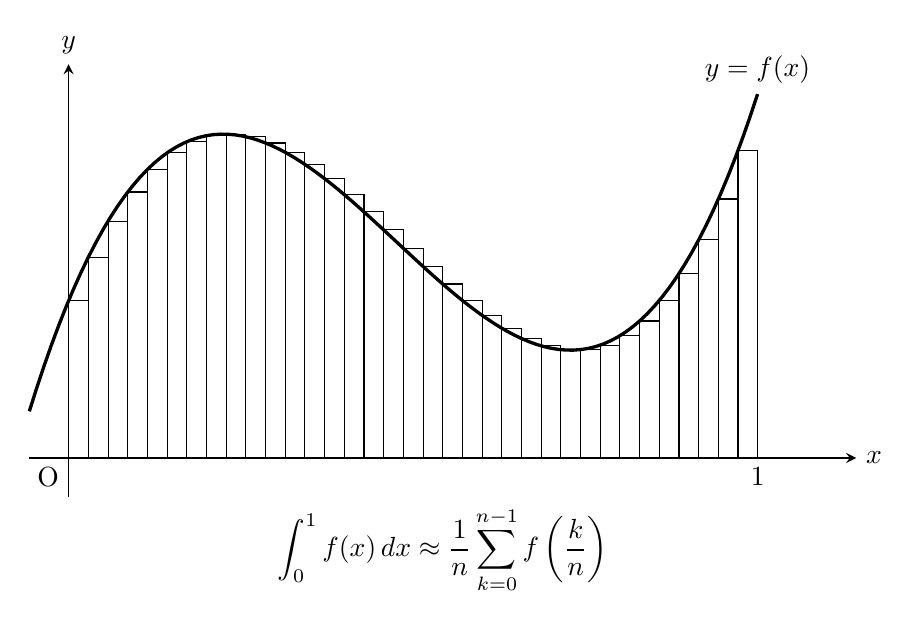
\begin{tikzpicture}[xscale=2.5]
 \coordinate[label=below  left:O] (O) at (-2,0); %原点O
 \coordinate (XS) at (-2.2,0); %x軸最小
 \coordinate (XL) at (2,0); %x軸最大
 \coordinate (YS) at (-2,-0.5); %y軸最小
 \coordinate (YL) at (-2,5); %y軸最大
 \draw[semithick,->,>=stealth] (XS)--(XL) node[right] {$x$}; %x軸
 \draw[semithick,->,>=stealth] (YS)--(YL) node[above] {$y$}; %y軸
 
 \draw[samples=100,domain=-2.2:1.5,very  thick]
   plot(\x,\x*\x*\x+\x*\x-2*\x+2) node[above] {$y=f(x)$};
   %y=f(x)のグラフ
 \foreach \t  in {-2,-1.9,...,1.5}
   \draw (\t,0)--(\t,\t*\t*\t+\t*\t-2*\t+2)--(\t+0.1,\t*\t*\t+\t*\t-2*\t+2)--(\t+0.1,0);
   %x=t,x=t+1の間の短冊
 \draw (1.5,0) node [below] {1}; %点(1,0)
 
 \draw ($(XS)!0.5!(XL)+(0,-0.5)$)
   node[below] {$\displaystyle\int_{0}^{1}f(x)\,dx \approx \frac{1}{n}\sum_{k=0}^{n-1}f\left(\frac{k}{n}\right)$};
   %図のx軸の中点+(0,-1)の位置に区分求積の式
\end{tikzpicture}

\[
  \begin{CD}
     0 @>>>  a  @>>>  b  @>>>  c  @>>>  0 \\
    @.     @VV{f}V  @VV{g}V  @VV{h}V   @. \\
     0 @>>>  a' @>>>  b' @>>>  c' @>>>  0
  \end{CD}
\]

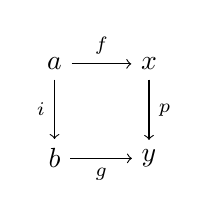
\begin{tikzpicture}[auto]
\node (a) at (0, 1.2) {$a$}; \node (x) at (1.2, 1.2) {$x$};
\node (b) at (0, 0) {$b$};   \node (y) at (1.2, 0) {$y$};
\draw[->] (a) to node {$\scriptstyle f$} (x);
\draw[->] (x) to node {$\scriptstyle p$} (y);
\draw[->] (a) to node[swap] {$\scriptstyle i$} (b);
\draw[->] (b) to node[swap] {$\scriptstyle g$} (y);
\end{tikzpicture}

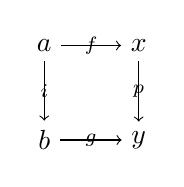
\begin{tikzpicture}
\node (a) at (0, 1.2) {$a$}; \node (x) at (1.2, 1.2) {$x$};
\node (b) at (0, 0) {$b$};   \node (y) at (1.2, 0) {$y$};
\draw[->] (a) to node {$\scriptstyle f$} (x);
\draw[->] (x) to node {$\scriptstyle p$} (y);
\draw[->] (a) to node[swap] {$\scriptstyle i$} (b);
\draw[->] (b) to node[swap] {$\scriptstyle g$} (y);
\end{tikzpicture}

%斜め線のやつ
\begin{center}
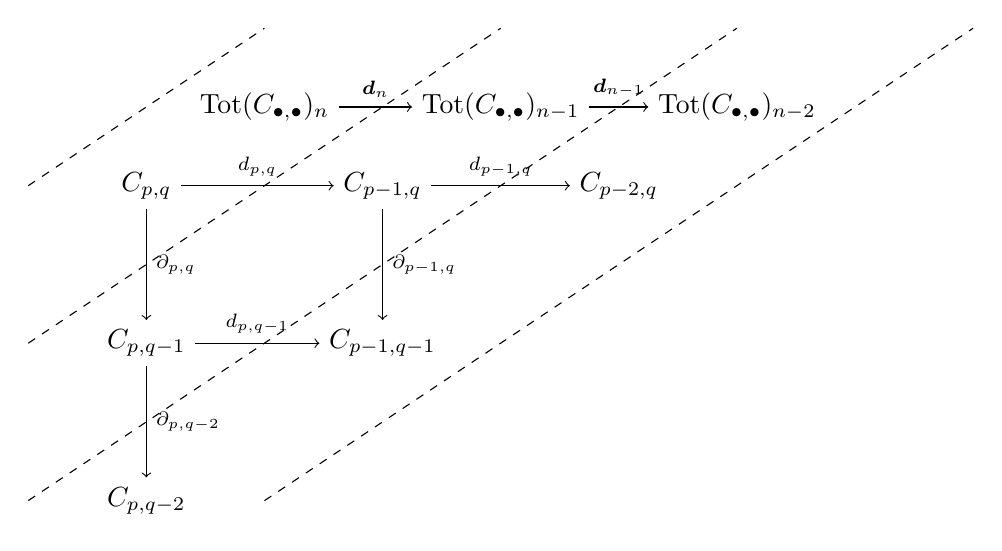
\begin{tikzpicture}[auto]
\node (a) at (0, 2) {$C_{p,q}$}; 
\node (b) at (3, 2) {$C_{p-1,q}$};
\node (c) at (6, 2) {$C_{p-2,q}$};
\node (d) at (0, 0) {$C_{p,q-1}$};   
\node (e) at (3, 0) {$C_{p-1,q-1}$};
\node (f) at (0, -2) {$C_{p,q-2}$};
\node (g) at (1.5, 3) {$\Tot(C_{\bullet, \bullet})_n$};
\node (h) at (4.5, 3) {$\Tot(C_{\bullet, \bullet})_{n-1}$};
\node (i) at (7.5, 3) {$\Tot(C_{\bullet, \bullet})_{n-2}$};
\draw[->] (a) to node {$\scriptstyle d_{p,q}$} (b);
\draw[->] (b) to node {$\scriptstyle d_{p-1,q}$} (c);
\draw[->] (b) to node {$\scriptstyle \partial_{p-1,q}$} (e);
\draw[->] (a) to node {$\scriptstyle \partial_{p,q}$} (d);
\draw[->] (d) to node {$\scriptstyle d_{p,q-1}$} (e);
\draw[->] (d) to node {$\scriptstyle \partial_{p,q-2}$} (f);
\draw[->] (g) to node {$\scriptstyle \bm{d}_n$} (h);
\draw[->] (h) to node {$\scriptstyle \bm{d}_{n-1}$} (i);
\draw [dashed] (-1.5, -2)--(7.5, 4);
\draw [dashed] (-1.5, 0)--(4.5, 4);
\draw [dashed] (-1.5, 2)--(1.5, 4);
\draw [dashed] (1.5, -2)--(10.5, 4);
\end{tikzpicture}
\end{center}

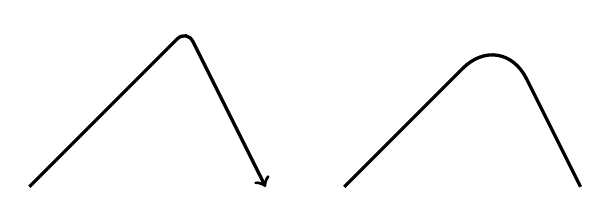
\begin{tikzpicture}
\draw[->,very thick,rounded corners = 5pt] (0,0) -- (2,2) -- (3,0) ;
\draw[very thick,rounded corners = 20pt] (4,0) -- (6,2) -- (7,0) ;
\end{tikzpicture}

\bigskip

\begin{tikzpicture}
\draw[->, rounded corners](0,2)--(5,2)--(5,0)--(0,0);
\end{tikzpicture}

\begin{center}
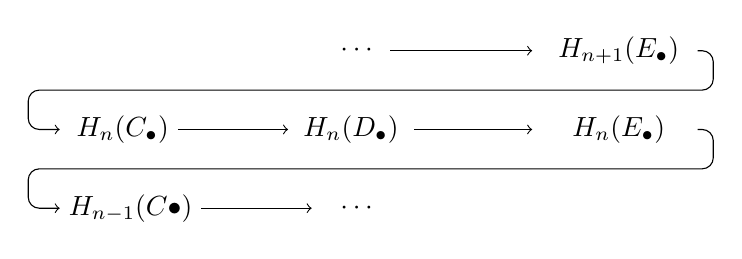
\begin{tikzpicture}[auto]
\node (a) at (4.2, 1) {$\cdots$};
\node (b) at (7.5, 1) {$H_{n+1} (E_{\bullet})$};
\node (c) at (1.2, 0) {$H_n (C_{\bullet})$};
\node (d) at (4.1, 0) {$H_n (D_{\bullet})$};
\node (e) at (7.5, 0) {$H_n (E_{\bullet})$};
\node (f) at (1.3, -1) {$H_{n-1} (C\bullet)$};
\node (a) at (4.2, -1) {$\cdots$};
\draw[->] (4.6, 1)--(6.4, 1);
\draw[->, rounded corners](8.5, 1)--(8.7, 1)--(8.7, 0.5)--(0, 0.5)--(0, 0)--(0.4, 0);
\draw[->] (1.9, 0)--(3.3, 0);
\draw[->] (4.9, 0)--(6.4, 0);
\draw[->, rounded corners](8.5, 0)--(8.7, 0)--(8.7, -0.5)--(0, -0.5)--(0, -1)--(0.4, -1);
\draw[->] (2.2, -1)--(3.6, -1);
\end{tikzpicture}
\end{center}

\bigskip

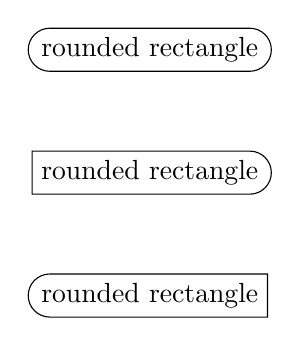
\begin{tikzpicture}
    \node (1) [draw, rounded rectangle] {rounded rectangle};
    \node (2) [below=of 1, draw, rounded rectangle, rounded rectangle west arc=0pt] {rounded rectangle};
    \node (3) [below=of 2, draw, rounded rectangle, rounded rectangle east arc=0pt] {rounded rectangle};
  \end{tikzpicture}

\begin{xy}
\xymatrix {
U \ar@/_/[ddr]_y \ar@{.>}[dr]|{\langle x,y \rangle} \ar@/^/[drr]^x \\
 & X \times_Z Y \ar[d]^q \ar[r]_p & X \ar[d]_f \\
 & Y \ar[r]^g & Z
}
\end{xy}

\[
\xymatrix{
x\ar@{|->}[r]&y
}\]

\[
\xymatrix{
F\ar[d]^{\sigma_0} & \subset & F(X)\ar[d]^{\tilde{\sigma}_F} & \ni & g(X)\ar@{|->}[d] & p(X)\ar@{|->}[d] \\
%\ar[d]で下線。^で右側に、_で左側に。
F'        & \subset & F'(X) & \ni & g^{\sigma_0}(x) & p^{\sigma_0}(X)}
\]

\begin{tikzpicture}[domain=0:4,samples=200,>=stealth]
  \draw[->] (-0.5,0)--(4.2,0) node[right] {$x$};
  \draw[->] (0,-0.5)--(0,2.2) node[above] {$y$};
  \draw plot (\x, {sqrt(\x)}) node[below] {$y=\sqrt{x}$};
  \draw (0,0) node[below left] {0};
\end{tikzpicture}

%sample=グラフをプロットする点の数（多いほど精度高くなる)
%stealth=x軸,y軸の矢印の部分
\begin{tikzpicture}[domain=0:4,samples=200,>=stealth] 
  \draw[->] (-3.5,0)--(3.5,0) node[right] {$x$};
  \draw[->] (0,-2.5)--(0,3.5) node[above] {$y$};
  \draw plot (\x, {abs(\x)}) node[right] {$y=|x|$};
  \draw (0,0) node[below left] {0};
\end{tikzpicture}

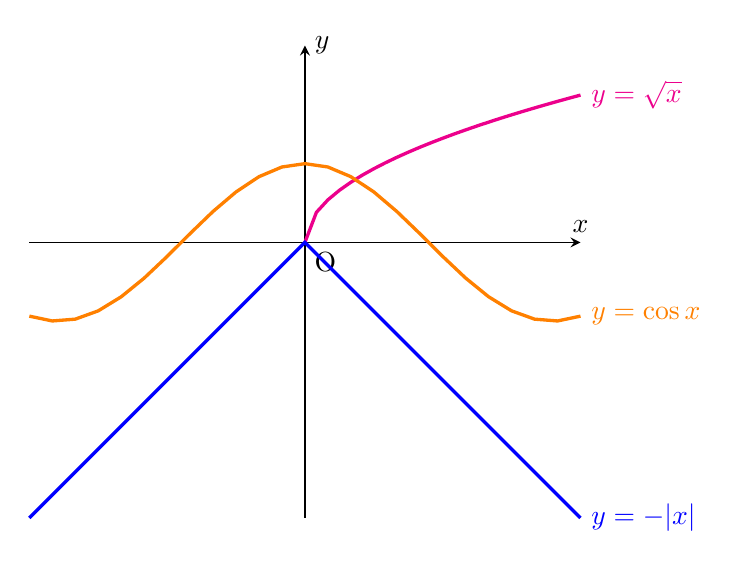
\begin{tikzpicture}
 \draw[->,>=stealth,semithick] (-3.5,0)--(3.5,0)node[above]{$x$}; %x軸
 \draw[->,>=stealth,semithick] (0,-3.5)--(0,2.5)node[right]{$y$}; %y軸
 \draw (0,0)node[below  right]{O}; %原点
 \draw[magenta,very  thick,domain=0:3.5] plot(\x,{sqrt(\x)})node[right]{$y=\sqrt{x}$};
 \draw[blue,very  thick,domain=-3.5:3.5] plot(\x,{-abs(\x)})node[right]{$y=-|x|$};
 \draw[orange,very  thick,domain=-3.5:3.5] plot(\x,{cos(\x r)})node[right]{$y=\cos{x}$};
\end{tikzpicture}

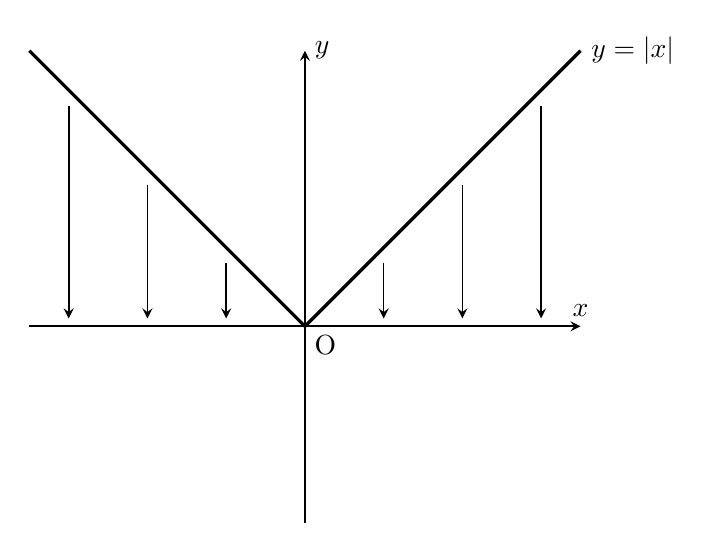
\begin{tikzpicture}
 \draw[->,>=stealth,semithick] (-3.5,0)--(3.5,0)node[above]{$x$}; %x軸
 \draw[->,>=stealth,semithick] (0,-2.5)--(0,3.5)node[right]{$y$}; %y軸
 \draw (0,0)node[below  right]{O}; %原点
 \draw[very  thick,domain=-3.5:3.5] plot(\x,{abs(\x)})node[right]{$y=|x|$};
 \draw[->,>=stealth,semithick] (1,0.8)--(1,0.1);
 \draw[->,>=stealth,semithick] (2,1.8)--(2,0.1);
 \draw[->,>=stealth,semithick] (3,2.8)--(3,0.1);
 \draw[->,>=stealth,semithick] (-1,0.8)--(-1,0.1);
 \draw[->,>=stealth,semithick] (-2,1.8)--(-2,0.1);
 \draw[->,>=stealth,semithick] (-3,2.8)--(-3,0.1);
\end{tikzpicture}

\begin{wrapfigure}{r}{0pt}
    \begin{tabular}{rr}

      \begin{minipage}[t]{0.2\linewidth}

      \begin{tikzpicture}
         \draw (0,0)--(3,0);
         \draw (1,1)--($(0,0)!(1,1)!(3,0)$);
\end{tikzpicture}
\caption{垂線}
      \end{minipage} &

      \begin{minipage}[t]{0.2\linewidth}
\begin{tikzpicture}
\draw (0,0) circle [x radius=2, y radius=1, rotate=30];
\end{tikzpicture}
\caption{円}
      \end{minipage}

    \end{tabular}
\end{wrapfigure}

\begin{tikzpicture}
  \coordinate [label=$A$] (a) at (0,0);
  \coordinate [label=$B$] (b) at (4,2);

  \fill (a) circle [radius=2pt];
  \fill (b) circle [radius=2pt];

  \fill ($(a)!0.2!(b)$) node [label=$P$] {} circle [radius=2pt];

  \draw [dashed] (a) -- (b);
  \draw [dashed] (1,0) -- (5,2);
\end{tikzpicture}


\begin{tikzpicture}
  \draw circle [radius=0.25];
  \foreach \r in {0.5,1,...,3} {
    \draw [orange, thick] (80:\r) arc [radius=\r, start angle=80, delta angle=-60];
  }
\end{tikzpicture}

\usetikzlibrary{positioning, graphs}
\pgfdeclarelayer{background}
\pgfsetlayers{background, main}

\begin{tikzpicture}
  \matrix [row sep=2em, column sep=2em,
           entity/.style={draw, circle,
                          minimum width=3em,
                          outer sep=3pt,
                          fill=white}] {
      \coordinate (instart) at (0,0);
    & \node [entity] (in0) { $u_{k-1}$ };
    & \node [entity] (in1) { $u_{k}$ };
    & \\

      \node [] (ststart) { $\cdots$ };
    & \node [entity] (st0) { $x_{k-1}$ };
    & \node [entity] (st1) { $x_{k}$ };
    & \node [] (stend) { $\cdots$ };\\

    & \node [entity] (ob0) { $y_{k-1}$ };
    & \node [entity] (ob1) { $y_{k}$ };
    & \coordinate (obend) at (0,0); \\
  };

  \graph {
      (ststart) -> (st0) -> (st1) -> (stend);
      (in0) -> (st0) -> (ob0);
      (in1) -> (st1) -> (ob1);
  };

  \coordinate (strect start) at (in0.north -| ststart.south west);
  \coordinate (strect end) at (st1.south -| stend.south east);

  \begin{pgfonlayer}{background}
    \fill [blue!20!white] (strect start) rectangle (strect end);
  \end{pgfonlayer}
\end{tikzpicture}

\bigskip

%to多様体より
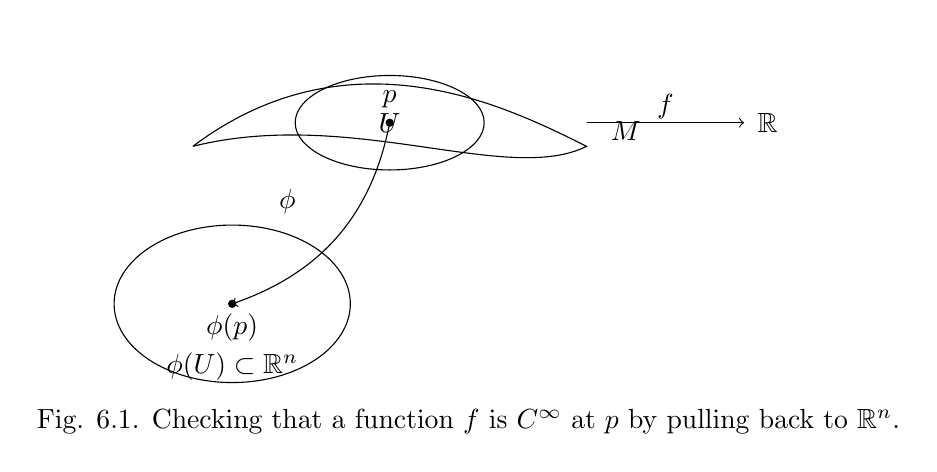
\begin{tikzpicture}
  % Draw the manifold M and the chart U
  \draw (0,2.5) .. controls (2,3) and (4,2) .. (5,2.5) .. controls (4,3) and (2,4) .. (0,2.5);
  \node at (5.5,2.7) {$M$};
  \draw (2.5,2.8) ellipse (1.2 and 0.6);
  \node at (2.5,2.8) {$U$};
  
  % Point p and its image under the chart phi
  \fill (2.5,2.8) circle (1.5pt);
  \node at (2.5,3.1) {$p$};
  \fill (0.5,0.5) circle (1.5pt);
  \node at (0.5,0.2) {$\phi(p)$};
  
  % Draw the arrow for phi and its image
  \draw[->] (2.5,2.8) to [bend left] (0.5,0.5);
  \node at (1.2,1.8) {$\phi$};
  
  % Draw the image of U under phi
  \draw (0.5,0.5) ellipse (1.5 and 1);
  \node at (0.5,-0.3) {$\phi(U) \subset \mathbb{R}^n$};
  
  % Draw the arrow for f
  \draw[->] (5,2.8) -- (7,2.8);
  \node at (6,3) {$f$};
  \node at (7.3,2.8) {$\mathbb{R}$};
  
  % Labels and caption
  \node at (3.5,-1) {Fig. 6.1. Checking that a function $f$ is $C^\infty$ at $p$ by pulling back to $\mathbb{R}^n$.};
\end{tikzpicture}

\begin{itembox}[l]{方針1の例題}
\begin{tasks}(2)
\task $\bigint (x+1)\sqrt{x-4}dx$
\task $\bigint \dfrac{x}{\sqrt{3+x}}dx$
\end{tasks}
\end{itembox}

\bf{解答}
\begin{multicols}{2}
a)\ $t=\sqrt{x-4} \mbox{と置き換えると}$

$\ x=t^2+4\ ,\ dx=2t\ dt $

\begin{eqnarray*}
&\mbox{（与式）}&=\int (t^2+4+1)t \cdot 2t\ dt\\
&&=2\int (t^4+5t^2) \ dt
\end{eqnarray*}

\vspace{0.5cm}

b)\ $t=\sqrt{3+x} \mbox{と置き換えると}$

$\ x=t^2-3\ ,\ dx=2t\ dt $

\begin{eqnarray*}
&\mbox{（与式）}&=\int \dfrac{t^2-3}{t}\cdot 2t \ dt\\
&&=2\int (t^2-3) \ dt
\end{eqnarray*}

\end{multicols} 




\section{たしざん}
たしざんを示す。
\begin{qbox}{たしざん}
    たしざんをする。
    \begin{equation*}
        \Biggl\lbrace
        \begin{alignedat}{2}
            1+1 &= 2 \\
            2 &= 1+1
        \end{alignedat}
    \end{equation*}
\end{qbox}

\begin{center}
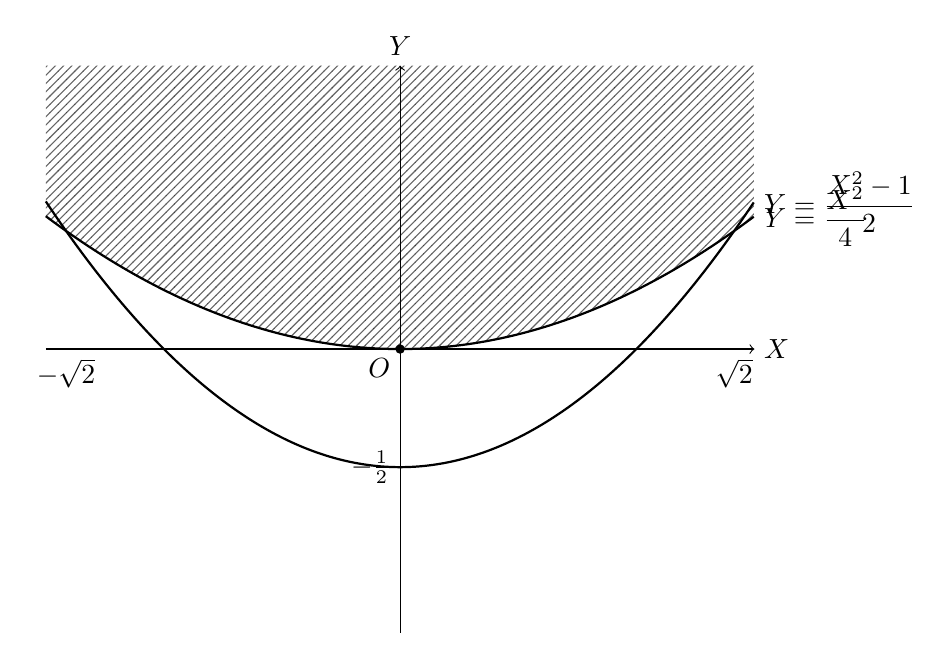
\begin{tikzpicture}[scale=3]
  % 軸
  \draw[->] (-1.5,0) -- (1.5,0) node[right] {$X$};
  \draw[->] (0,-1.2) -- (0,1.2) node[above] {$Y$};
  
  % 放物線 Y = X^2/4
  \draw[thick,domain=-1.5:1.5,samples=200] 
    plot(\x,{\x*\x/4}) node[right] {$Y=\dfrac{X^2}{4}$};
    
  % 放物線 Y = (X^2 - 1)/2
  \draw[thick,domain=-1.5:1.5,samples=200] 
    plot(\x,{(\x*\x-1)/2}) node[right] {$Y=\dfrac{X^2-1}{2}$};
    
  % 斜線部分の塗りつぶし
  \begin{scope}
    \clip (-1.5,-1.2) rectangle (1.5,1.2);
    \clip (-1.5,-1.2) rectangle (1.5,1.2);
    \fill[pattern=north east lines,opacity=0.6]
      plot[domain=-1.5:1.5,samples=200] (\x,{\x*\x/4}) --
      (1.5,1.2) -- (-1.5,1.2) -- cycle;
  \end{scope}

  % 点O
  \fill (0,0) circle (0.02) node[below left] {$O$};
  
  % 軸の目盛り
  \draw (1.414,0) node[below] {$\sqrt{2}$};
  \draw (-1.414,0) node[below] {$-\sqrt{2}$};
  \draw (0,-0.5) node[left] {$-\tfrac{1}{2}$};
\end{tikzpicture}
\end{center}


\begin{center}
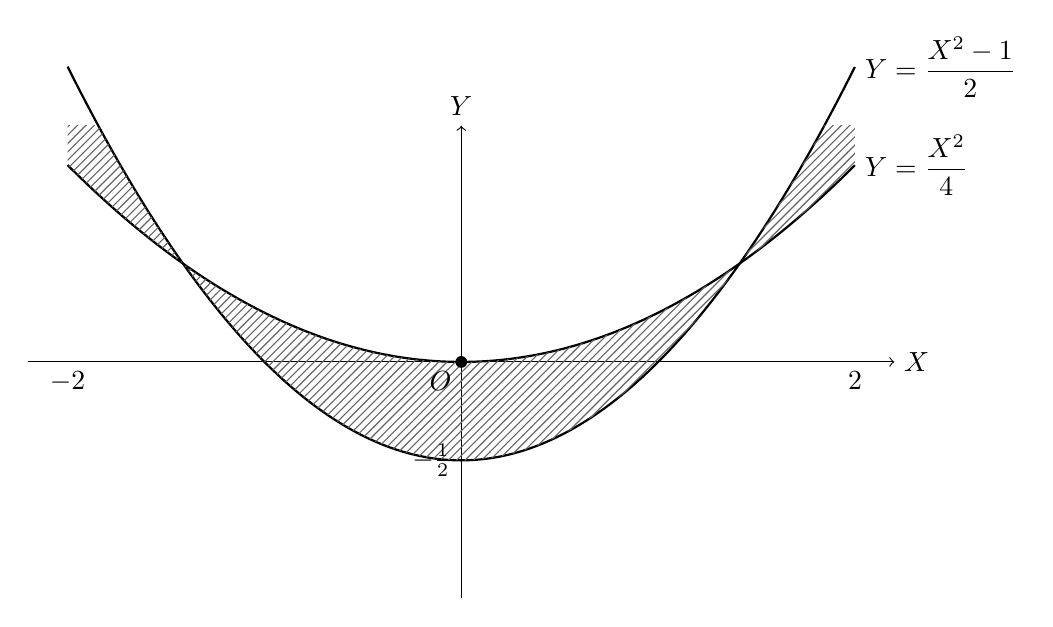
\begin{tikzpicture}[scale=2.5]
  % 軸
  \draw[->] (-2.2,0) -- (2.2,0) node[right] {$X$};
  \draw[->] (0,-1.2) -- (0,1.2) node[above] {$Y$};
  
  % 放物線 Y = X^2/4
  \draw[thick,domain=-2:2,samples=200] 
    plot(\x,{\x*\x/4}) node[right] {$Y=\dfrac{X^2}{4}$};
    
  % 放物線 Y = (X^2 - 1)/2
  \draw[thick,domain=-2:2,samples=200] 
    plot(\x,{(\x*\x-1)/2}) node[right] {$Y=\dfrac{X^2-1}{2}$};
    
  % 斜線部分の塗りつぶし（2つの放物線の間）
  \begin{scope}
    \clip (-2,-1.2) rectangle (2,1.2);
    \fill[pattern=north east lines,pattern color=black!60]
      plot[domain=-2:2,samples=200] (\x,{\x*\x/4}) -- plot[domain=2:-2,samples=200] (\x,{(\x*\x-1)/2}) -- cycle;
  \end{scope}

  % 点O
  \fill (0,0) circle (0.03) node[below left] {$O$};
  
  % 軸の目盛り
  \draw (2,0) node[below] {$2$};
  \draw (-2,0) node[below] {$-2$};
  \draw (0,-0.5) node[left] {$-\tfrac{1}{2}$};
\end{tikzpicture}
\end{center}



\begin{center}
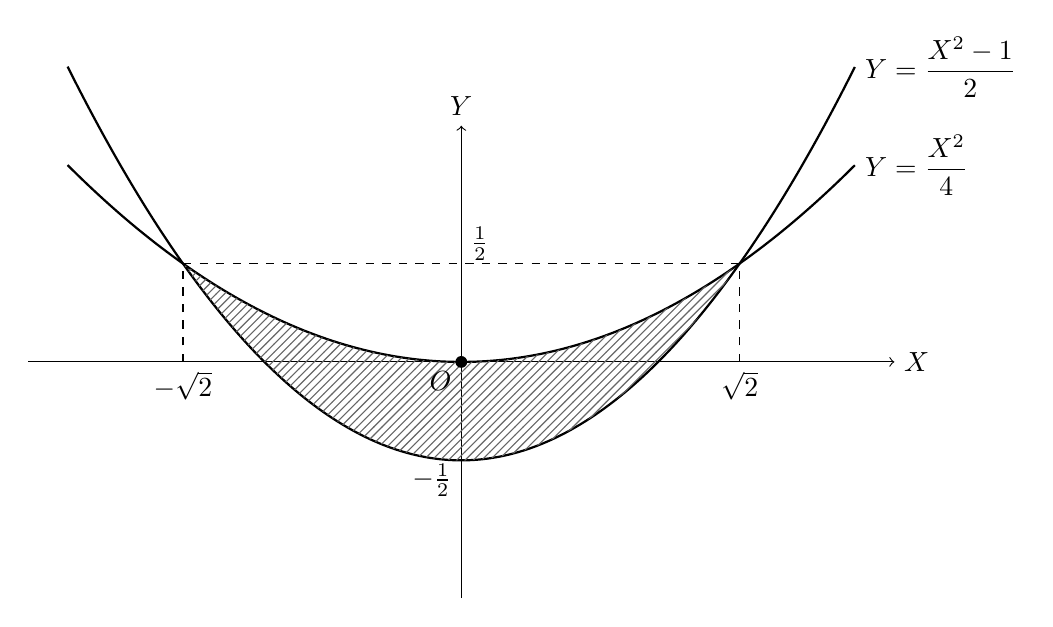
\begin{tikzpicture}[scale=2.5]
  % 軸
  \draw[->] (-2.2,0) -- (2.2,0) node[right] {$X$};
  \draw[->] (0,-1.2) -- (0,1.2) node[above] {$Y$};
  
  % 放物線 Y = X^2/4
  \draw[thick,domain=-2:2,samples=200] 
    plot(\x,{\x*\x/4}) node[right] {$Y=\dfrac{X^2}{4}$};
    
  % 放物線 Y = (X^2 - 1)/2
  \draw[thick,domain=-2:2,samples=200] 
    plot(\x,{(\x*\x-1)/2}) node[right] {$Y=\dfrac{X^2-1}{2}$};
    
  % 斜線部分（-√2 <= x <= √2 の範囲）
  \begin{scope}
    \clip (-1.414,-1.2) rectangle (1.414,1.2); % √2 ≈ 1.414
    \fill[pattern=north east lines,pattern color=black!60]
      plot[domain=-1.414:1.414,samples=200] (\x,{\x*\x/4}) --
      plot[domain=1.414:-1.414,samples=200] (\x,{(\x*\x-1)/2}) -- cycle;
  \end{scope}

  % 点O
  \fill (0,0) circle (0.03) node[below left] {$O$};
  
  % 軸の目盛り
  \draw (0,0.6) node[right] {$\frac{1}{2}$};
  \draw (1.414,0) node[below] {$\sqrt{2}$};
  \draw (-1.414,0) node[below] {$-\sqrt{2}$};
  \draw (0,-0.6) node[left] {$-\tfrac{1}{2}$};

  % 点線
  \draw[dashed] (-1.414,0) -- (-1.414,0.5);
  \draw[dashed] (1.414,0) -- (1.414,0.5);
  \draw[dashed] (-1.414,0.5) -- (1.414,0.5);
\end{tikzpicture}
\end{center}



documentclassのところにdvipdfmxを入れないと出力されないため注意↓

\vspace{5zw}
\begin{wrapfigure}{r}{0pt} %図形を右側に
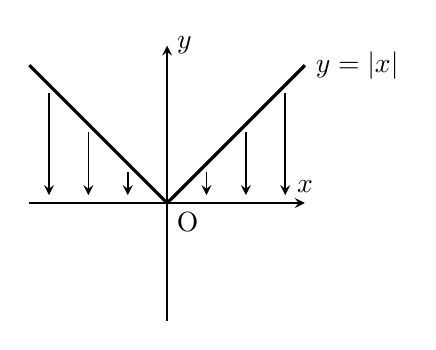
\begin{tikzpicture}
 \draw[->,>=stealth,semithick] (-1.75,0)--(1.75,0)node[above]{$x$}; %x軸
 \draw[->,>=stealth,semithick] (0,-1.5)--(0,2)node[right]{$y$}; %y軸
 \draw (0,0)node[below  right]{O}; %原点
 \draw[very  thick,domain=-1.75:1.75] plot(\x,{abs(\x)})node[right]{$y=|x|$};
 \draw[->,>=stealth,semithick] (0.5,0.4)--(0.5,0.1);
 \draw[->,>=stealth,semithick] (1.0,0.9)--(1.0,0.1);
 \draw[->,>=stealth,semithick] (1.5,1.4)--(1.5,0.1);
 \draw[->,>=stealth,semithick] (-0.5,0.4)--(-0.5,0.1);
 \draw[->,>=stealth,semithick] (-1.0,0.9)--(-1.0,0.1);
 \draw[->,>=stealth,semithick] (-1.5,1.4)--(-1.5,0.1);
\end{tikzpicture}
\end{wrapfigure}
$M$ は $\mathbb{R}^2$ の部分空間なのでHausdorff空間となる.

次に, 関数$y = |x|$ を$x$軸に射影する.

写像$\varphi$ を
\[\begin{array}{rccc}
\varphi \colon & M & \longrightarrow   & \mathbb{R} \\
        & \rotatebox{90}{$\in$} & & \rotatebox{90}{$\in$} \\
        & (x,|x|) & \longmapsto & x
\end{array}\]

とすると, 全単射は明らか. 射影なので連続. 逆写像$\varphi^{-1}$ の連続性も明らか. よって$\varphi$ は同相写像. 
以上より$M$は位相多様体.

\vspace{5zw}

{\HUGE
$$
\colondash
$$
$$
\coloneqq
$$
$$
\coloneq
$$
$$
\Coloneqq
$$
$$
\Coloneq
$$
$$
\colonsim \\
\Colonsim \\
\colonapprox \\
\Colonapprox \\
\dashcolon \\
\Dashcolon \\
\eqqcolon \\
\Eqqcolon \\
\Simcolon \\
\approxcolon \\
\Approxcolon \\
$$
}

───\textcircled{\scriptsize 1}

\newcommand{\mrk}[1]{
\raisebox{-3pt}{
\!\!
\begin{tikzpicture}[x=1pt,y=1pt,line width=1pt]
\draw (0,0) ellipse (4.5 and 6);
\draw (0,0) node{
\usefont{T1}{phv}{m}{n}
\fontsize{9pt}{0}
\selectfont #1 };
\end{tikzpicture}}}

\end{document}
